\documentclass{article}
\usepackage{graphicx}
\usepackage{amsmath}
\usepackage{listings}
\usepackage{caption}
\usepackage[hidelinks]{hyperref}
\setlength{\parindent}{0pt}


\begin{document}

    \begin{titlepage}
    \vbox{ }
    \vbox{ }
    \begin{center}
        % Course
        
\includegraphics[width=1\textwidth]{./images/ifi.png}\\[1cm]
        \textsc{\Large IN4050 - Introduction to Artificial Intelligence and Machine Learning}\\[0.5cm]
        \vbox{ }
        
        % Title
        { \huge \bfseries Mandatory Assignment \#1}\\[0.4cm]
        
        \large
        \emph{Author:}\\
            Kjetil K. Indrehus \\[0.9cm]
           
            \large kjetiki@ifi.uio.no \\[0.1cm]
            (username: kjetiki)
        \vfill
        
        {\large\today}
    \end{center}
\end{titlepage}
    
    \section{Usage}

    All code can by run by using the Jupyter notebook called \textit{Assignment1.ipynb} file. \\

    This project is developed with Python virtual environment.  
    All packages required are in the \textit{requirements.txt}.
    With VSCode, use the following guide to setup the virtual environment \url{https://code.visualstudio.com/docs/python/environments}. \\

    After the environment are created, you should have a \textit{.venv} directory in the root folder. 
    Make sure to select the environment when using the notebook. 

    \newpage

    \section{Exhaustive search}

    My implemented the Exhaustive Search algorithm has the following steps: 

    \begin{itemize}
        \item Creating variables for storing the best solutions.
        \item Iterate over each city, and make that city the starting point. 
        \begin{itemize}
            \item Generate all possible permutations of the list of cities without the starting city. Each permutation is the \textit{middle route} and does not contain the end and the start city.
            \item For each permutation, create a route by taking the starting city + the \textit{middle route} + start city again. The length of the route be the amount of cities that are allowed + 1 for the end city. (For example 6 cities to visit $\to$ route will be 7 cities long, because we always have to return)
            \item Calculate the distance for the route
            \item If the distance is lower, set the route as the best route. 
        \end{itemize}
    \end{itemize}


    \subsection{Shortest route for 10 cities}

    The following route was the shortest for 10 cities: 
    \[
    \begin{aligned}
        \text{Copenhagen} \to \text{Hamburg} \to \text{Brussels} \to \text{Dublin} \to \text{Barcelona} \to \\
        \text{Belgrade} \to \text{Istanbul} \to \text{Bucharest} \to \text{Budapest} \to \text{Berlin} \to \text{Copenhagen}
    \end{aligned}
    \]

    The total time it took was: \textbf{0:00:11.611775} (11.611775 seconds)

    This image shows the route:

    \begin{figure}[h!]
        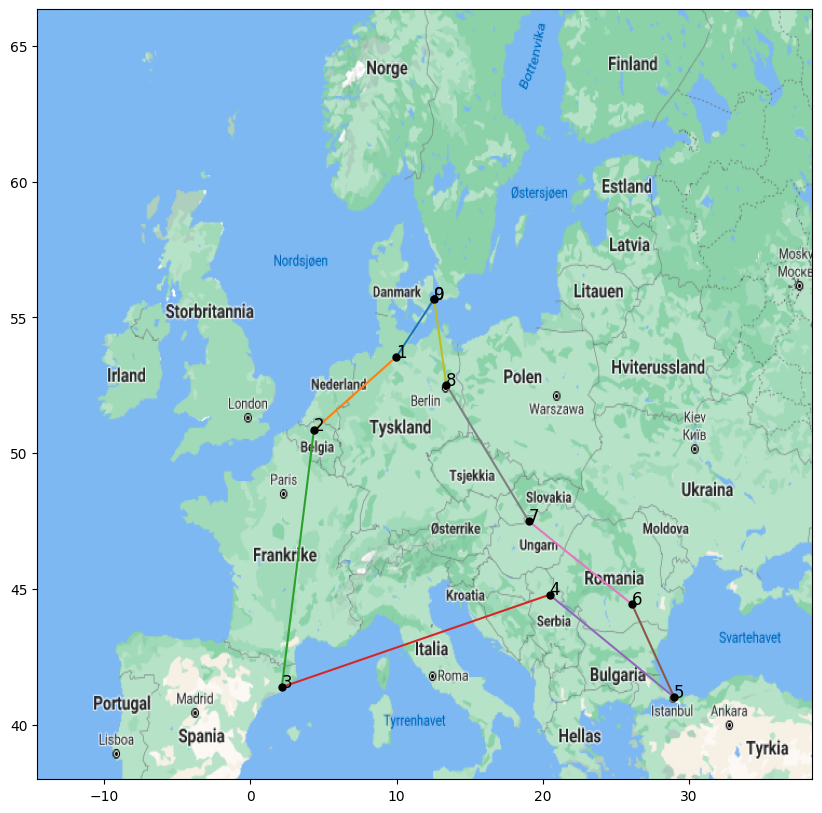
\includegraphics[width=7cm]{images/exhaustive_search_result_10_cities.png}
        \centering
        \caption{Exhaustive Search 10 cities plotted route}
    \end{figure}

    \newpage

    \subsection{Approximation for 24 cities}

    By running the code multiple times, I found out the following: 

    \begin{enumerate}
        \item 6 cities $\to$ 0:00:00.001707 $\to$ $P = 6! = 720$ routes to be checked 
        \item 8 cities $\to$ 0:00:00.123331 $\to$ $P = 8! = 40320$ routes to be checked 
        \item 9 cities $\to$ 0:00:01.006485 $\to$ $P = 9! = 362880$ routes to be checked 
        \item 10 cites $\to$ 0:00:10.756498 $\to$ $P = 10! = 3628800$ routes to be checked 
    \end{enumerate}

    I also tried with 12 cities, but it took more then 3 minutes. Clearly the growth is exponential with the permutations done for each route. 

    With 24 cites, there are $24! = 6,204484017*10^{23}$ possible routes!
    To approximate how long it would have taken for all the routes, I check how long it takes to generate one permutation and check it: 

    \[
    \text{Time per permutation}_n = \frac{\text{Total time}}{n!}
    \]

    For each test, I calculate how long it took for each permutation: 

    \[
    \text{Time per permutation for 6 cities} = \frac{0.001707}{720} \approx 2.3708 \times 10^{-6} \text{ s/route}
    \]

    \[
    \text{Time per permutation for 8 cities} = \frac{0.123331}{40320} \approx 3.0588 \times 10^{-6} \text{ s/route}
    \]

    \[
    \text{Time per permutation for 9 cities} = \frac{1.006485}{362880} \approx 2.7736 \times 10^{-6} \text{ s/route}
    \]

    \[
    \text{Time per permutation for 10 cities} = \frac{10.756498}{3628800} \approx 2.9642 \times 10^{-6} \text{ s/route}
    \]

    With this, I assume that each permutation will take the average amount of time to generate a permutation: \[2.7918\times10^{-6} \text{ s/route} \]
    Note that this might not always be correct, but I think this is a good way to approximate how long it would have taken for 24 cities. 

    Now, using this average, all me need to do is multiply the amount of permutations with the average time for each permutation to be generated: 

    \[
    \begin{aligned}
        \text{Total Time} &= 6.204484017 \times 10^{23} \times 2.7918\times10^{-6} \text{ s/route} \\
                          &= 1.73217 \times 10^{18} \text{ s}
    \end{aligned}
    \]

    To make the approximation more readable, I used a python library. 
    It has a function to make seconds into a more readable format. Link to docs: 
    \url{https://humanfriendly.readthedocs.io/en/latest/api.html#humanfriendly.format_timespan} \newline

    Using the function to get the total time in a readable format, shows how long time 24 cities with exhaustive search would have taken: \textbf{55077648046 years, 20 weeks and 4 days}.

    \section{Hill Climbing}

    Hill Climbing is an algorithm that combines randomness and greedy search into a single algorithm.
    This is how my implementation works:
    \begin{itemize}
        \item Create a random initial route (valid route only)
        \item Store the best route in a variable. For each of the 20 runs: 
        \begin{itemize}
            \item Create a neighbor solution by swapping two random cities. The cities swapped are not the start city. 
            \item Evaluate this neighbor solution, and set it as the best route, if the distance is smaller
        \end{itemize}
    \end{itemize}


    There is a lot of different ways to create a random neighbor solution. By experimenting, it turns out that swapping to cities on the current best solution is a good idea. 
    It converges towards a better solution. It is still important to run it 20 times, because it has a random element to it. 

    \subsection{Performance compared to Exhaustive Search (10 cities)}

    Hill climbing compared to Exhaustive Search, does not look at every solution. This means both that it is less likely to find the best solution.
    With 10 cities are the total search space much smaller. It took $\sim1.6$ seconds to find the best distance 7486.309 km. Even though we found the same solution as Exhaustive Search, there is a difference in time spent.
    Exhaustive Search used  $\sim13.48$ seconds (compared to the   $\sim1.6$ seconds). \\

    The only flaw with the Hill Climbing algorithm, is that we need to run it multiple times to get a deterministic result. This is because the Hill Climbing algorithm has a random element to it. 
    20 runs seems to be enough to get the same best route as exhaustive search 

    \subsection{Result for 10 and 24 cities (20 runs each)}

    The following is a table showing the result for both runs:

    \begin{table}[ht]
        \centering
        \resizebox{\textwidth}{!}{
            \begin{tabular}{|c|c|c|c|c|c|}
                \hline
                \textbf{Number of Cities} & \textbf{Best Distance} & \textbf{Average Distance} & \textbf{Worst Distance} & \textbf{Std. Deviation} & \textbf{Time Taken (s)} \\ \hline
                \textbf{10 Cities}        & 7486.31     & 7825.79     & 8421.35     & 405.37            & $\sim1.6$             \\ \hline
                \textbf{24 Cities}        & 13347.75    & 15083.53    & 17177.85    & 1079.74           & $\sim2.2$             \\ \hline
            \end{tabular}
        }
        \caption{Hill Climbing results for 10 and 24 cities (20 runs each)}
    \end{table}
    

    Images below are plotted routes of the best routes from a run: 

    \begin{figure}[ht]
        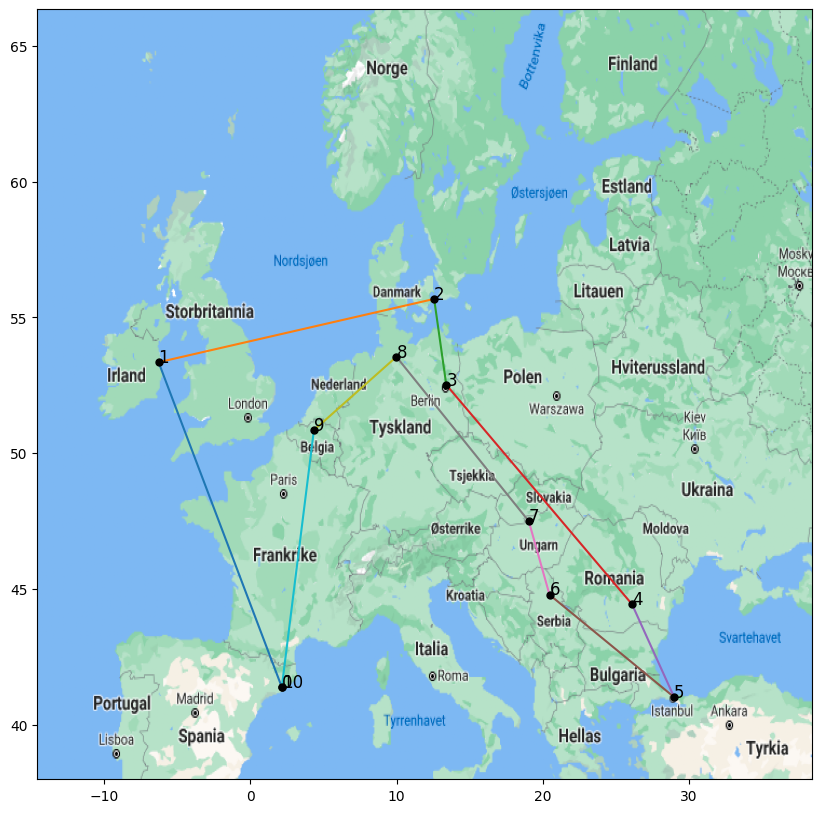
\includegraphics[width=7cm]{images/hill_climb_10_cities.png}
        \centering
        \caption{Hill climb 10 cities plotted route}
    \end{figure}


    \begin{figure}[ht]
        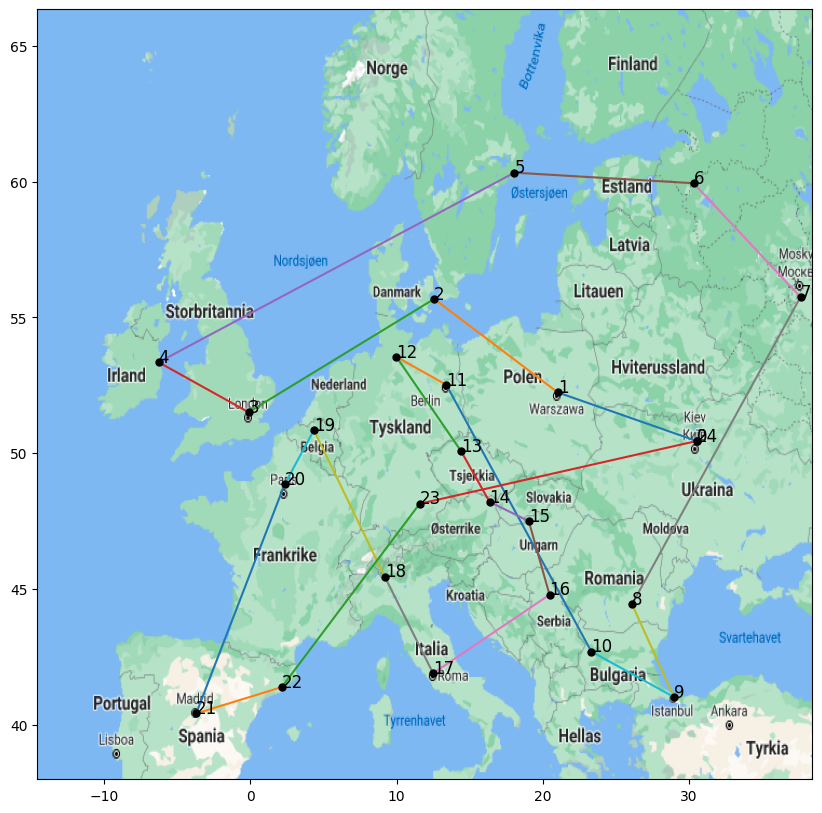
\includegraphics[width=7cm]{images/hill_climb_24_cities.png}
        \centering
        \caption{Hill climb 24 cities plotted route}
    \end{figure}

    \section{Genetic algorithm}

    Genetic algorithm is very inspired by evolutions, and is very useful for both search problems where a combination of exploration and exploitation is useful.
    There is many different tricks and variations when it comes to the algorithm. Based on the problem, the developer can implement domain specific elements to the algorithm. For example, picking a specific mutation method based on the understanding of the problem. \\
    
    Genetic algorithm is flexible, but still follows the general scheme. For each part of the scheme, I will explain what I did, some experimenting I did and reason on why I choose the given method for the traveling salesman problem.

    \begin{figure}[ht]
        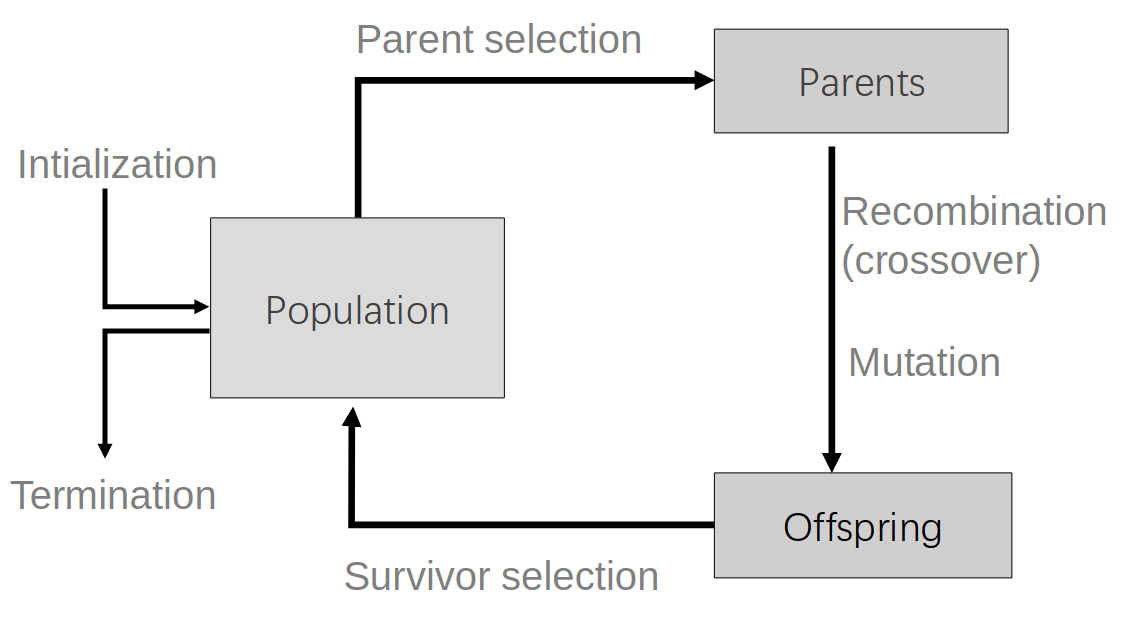
\includegraphics[width=7cm]{images/ga_scheme.png}
        \centering
        \caption{GA scheme for reference}
    \end{figure}


    \subsection{Create initial population and population size}

    There are two key points for generating a starting population. First, each route generated has to be a valid route. 
    Secondly, diversity is key to avoid going into a local optima. Start city is not that important. A route could have the same distance and different start city. 
    It is the order that will matter the most. 

    \subsection{Fitness}

    Fitness express how well a solution is. For the traveling salesman problem, I chose the inverse of the distance. This means that if the distance is smaller, the better will the fitness be.
    This fits well with what the goal is: find the route with the minimal distance.

    \subsection{Parent Selection}

    From the population, we select a set of parents that will together create offspring. 
    For the problem, I chose roulette wheel selection. This method will allow the fittest routes to be more likely to become parents. 
    This also allows for more exploration, because less fit routes will also be picked. \\ 

    The probability for each item to be picked is the percentage of its own fitness over the sum of fitness for the whole population. This is also known as fitness sharing. 

    \subsection{Crossover}

    All of the parents will randomly be selected for creating each offspring. I have chosen that the total amount of offspring should be 30\% of the total population. 
    This will allow the a lot of new solutions to come in and be part of selections. It is also low enough to allow the new offspring to completely take over the population majority.\\

    After looking over all possible crossover methods, and reading on what options there are. The method I picked in the end was: Edge Recombination Crossover. 
    This is a method that was shown in a group session by the TAs. It is often used in networking problems. It uses two parents and creates a new offspring with similar paths. 
    It fits the problem very well: we want to use the offspring to be similar to both parents, while being unique. \\

    It is implemented by creating similarity matrixes, based on what edges each city is connected to. 
    See the following algorithm for implementation details: \url{https://en.wikipedia.org/wiki/Edge_recombination_operator}
    

    \subsection{Mutation}

    A typical way to include some more exploration for the solution is by mutation. A mutations is a small change. 
    It was not clear how often it was good to mutate the offspring, but after testing with 10\%, 20\% and 25\% mutation rate, I ended up using 20\%. 
    The reasoning is that I saw on the fitness graph that it plateaus if the mutation probability was 10\%. It seems to be changing too much when the percentage was 25\%. 

    \subsection{Survivor Selection}

    When selecting surviving routes, we want to keep the best solutions. To make this happen, I implement elitism. 
    After offspring and population is combined, then we take the top 10\% of the most fit solutions. \\
    
    
    The original idea was fill the rest of the slots by shuffling the remaining solutions and pick then until we have a population with the desired size.
    This turned out to convert very fast, and get stuck in local optima. \\

    \begin{figure}[ht!]
        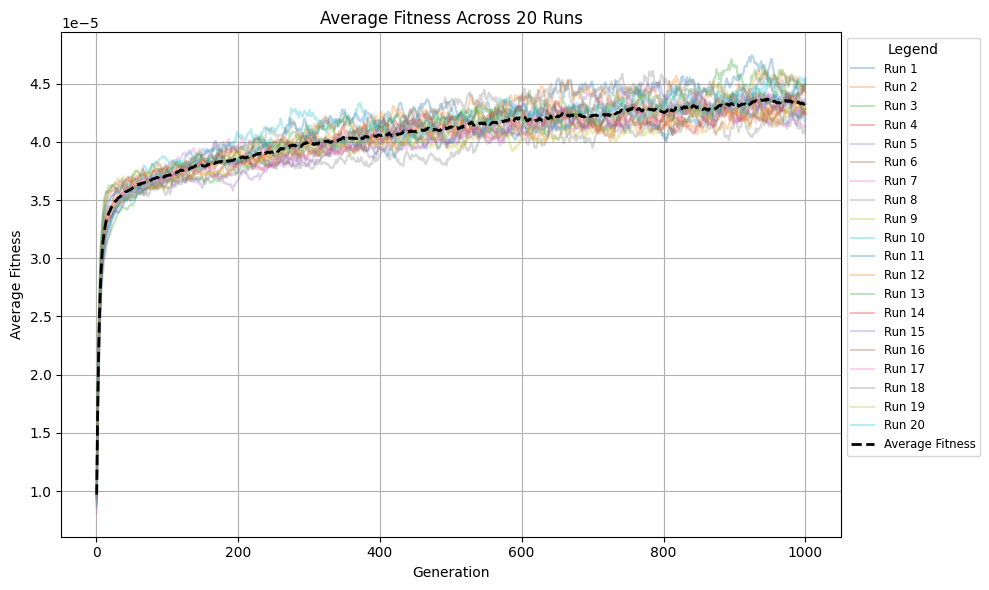
\includegraphics[width=12cm]{images/with_bad_inital_population.png}
        \centering
        \caption{Screenshot from development where GA for 24 cities are converging too fast}
    \end{figure}


    I changed the way to select the rest of the remaining population, by again using roulette selection by fitness sharing. The fitness sharing happens with the remaining population. 
    This techniques ensures that there is more likely to pick better solutions but also keep the distribution between the bad and worst solution. 
    When the fitness for every solution is about the same, then all will solutions will have about the same probability. See results for 24 cities to see the improved convergence.

    \subsection{Termination}

    This loop will continue forever until it hits some condition to stop. My initial idea was to terminate if the same best route was for x generations in a row.
    Instead I made the GA run through a given amount of iterations. My solutions converges quite quickly, but will only find the best solution after exploring a lot more after convergence. 

    \newpage

    \subsection{Results: 10 cities}

    For 10 cities GA ran with a population size of 200, and maximum 200 generations.

    \begin{figure}[ht!]
        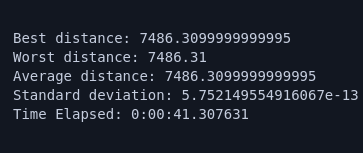
\includegraphics[width=7cm]{images/ga_10_cities_summary.png}
        \centering
        \caption{Summary of 20 runs, 10 cities from Notebook}
    \end{figure}

    We see that the algorithm is able to find the best route. It does so in less than a minute.
    The fitness graph shows that it rapidly converges within the first 50 generations.

    \begin{figure}[ht!]
        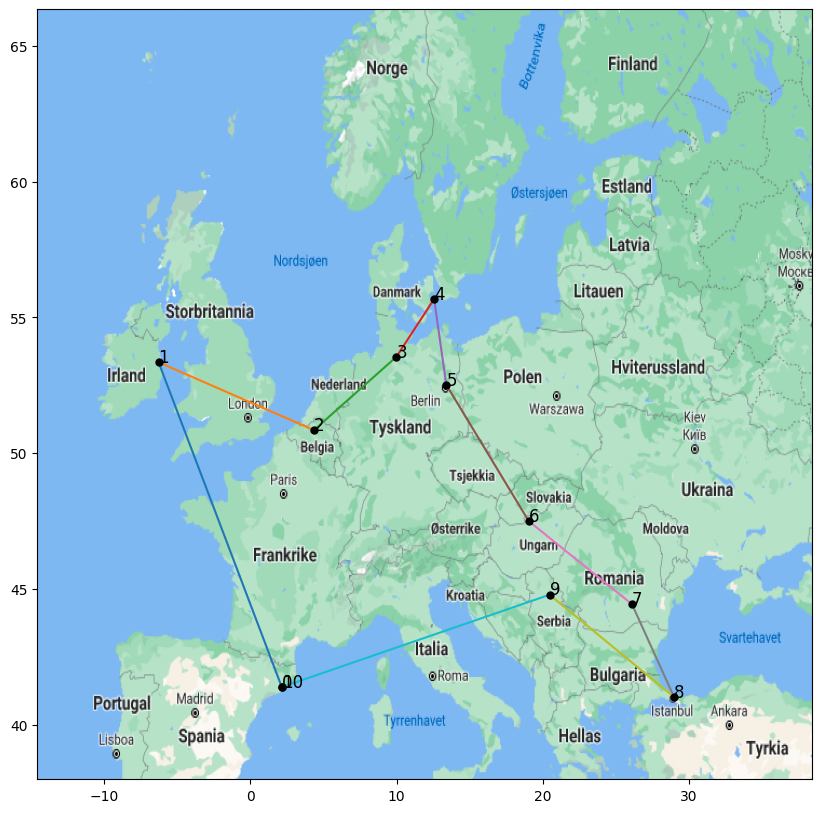
\includegraphics[width=10cm]{images/ga_10_cities.png}
        \centering
        \caption{GA result for 10 cities}
    \end{figure}

    \begin{figure}[ht!]
        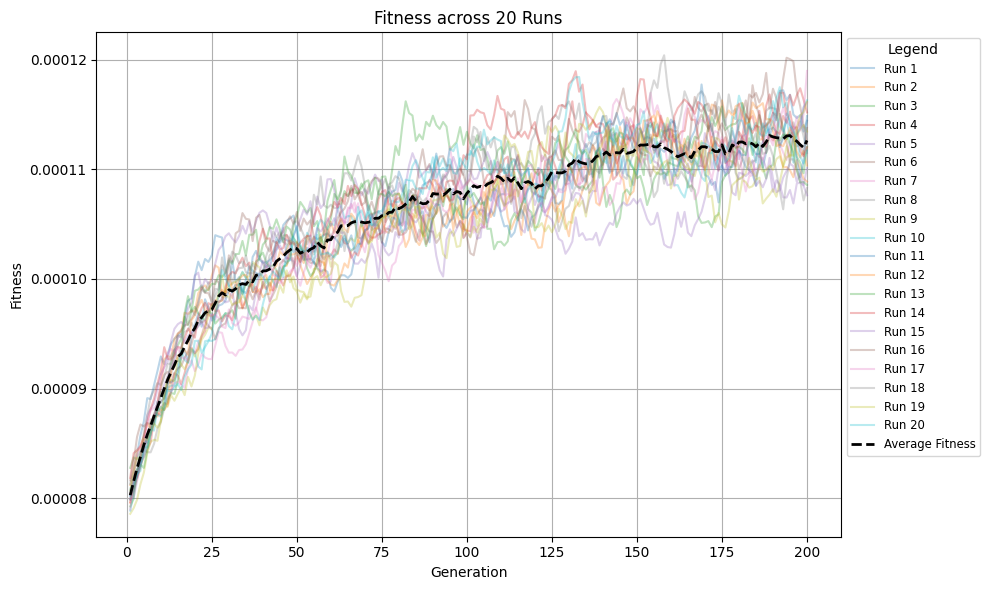
\includegraphics[width=12cm]{images/ga_10_cities_avg_graph.png}
        \centering
        \caption{Average Fitness for 10 cities and 20 runs}
    \end{figure}


    \newpage


    \subsection{Results: 24 cities}

    For 24 cities, the GA was ran with a population size of 300 and maximum 1000 generations.

    \begin{figure}[ht!]
        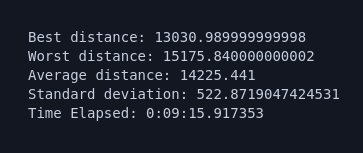
\includegraphics[width=7cm]{images/ga_24_cities_summary.png}
        \centering
        \caption{Summary of 20 runs, 24 cities from Notebook}
    \end{figure}

    \begin{figure}[ht!]
        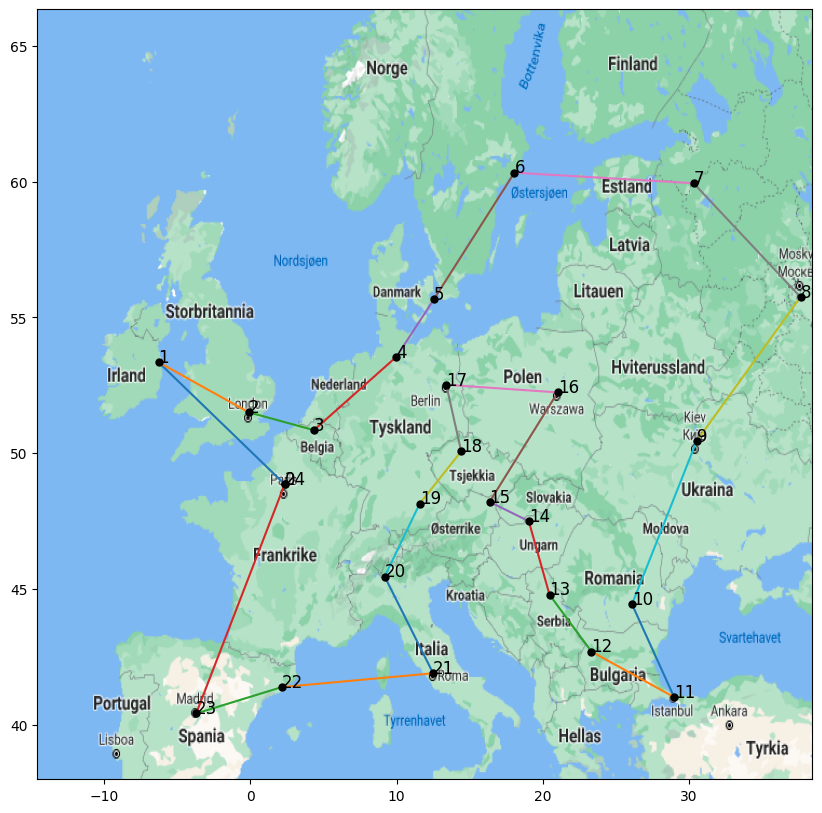
\includegraphics[width=9cm]{images/ga_24_cities.png}
        \centering
        \caption{GA result for 24 cities}
    \end{figure}

    For the fitness graph for 24 cities, it is able to slowly converge towards the best solution, instead of getting stuck at a local optima:

    \begin{figure}[ht!]
        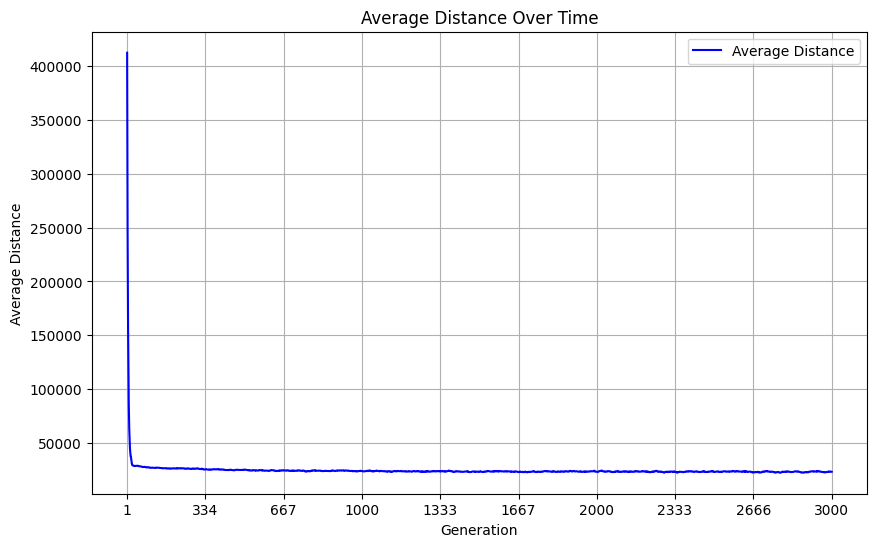
\includegraphics[width=12cm]{images/ga_24_cities_avg_graph.png}
        \centering
        \caption{Average Fitness for 24 cities and 20 runs}
    \end{figure}

    \newpage

    \subsection{GA compared to Exhaustive Search (24 cities)}

    Exhaustive search will go trough every possible permutation. For 24 cities there are 24! permutations. 
    To approximate how many routes the genetic algorithm is through on a single run:

    \begin{enumerate}
        \item The initial population consists of 500 unique solutions.
        \item We create new offspring which is 30\% of the total population.
        \item Assuming 80\% of the offspring are new, we can calculate the number of new routes processed.
    \end{enumerate}

    Let \(P\) be the total population size, \(O\) be the offspring size.
    Assuming 80\% of the offspring are new, the number of new offspring generated is:
    \[
    N = 0.8 \times O = 0.8 \times (0.3 \times P) = 120
    \]

    The genetic algorithm continues to iterate through generations. Assuming \(G\) is the number of generations run, the total number of routes processed by the genetic algorithm can be approximated as:
    \[
    \text{Total Routes Processed} \approx P_{\text{initial}} + G \times N
    \]

    For 500 start population, 1000 generations and 120 new populations each time: 
    \[
    \text{Total Routes Processed} \approx 500 + 1000 \times 120 \approx 120500 \text{ routes checked}
    \]

    This is much less then all the routes that have to be checked by exhaustive search.
    Even if \textit{all} of the start populations are replaced each time, it would still be significantly less then Exhaustive Search
    \[
    500 + 1000 \times 500 \ll 24!
    \]

    The genetic algorithm checks significantly fewer routes then exhaustive search. Note that this approximation is only an approximation. 
    This might be the wrong way of approximating, but it shows that genetic algorithm is much better than exhaustive search. 

\end{document}